%%%%%%%%%%%%%%%%%%%%%%%%%%%%%%%%%%%%%%%%%%%%%%%%%%%%%%%%%%%%%%%%%%%%%%
% Overleaf (WriteLaTeX) Example: Molecular Chemistry Presentation
%
% Source: http://www.overleaf.com
%
% In these slides we show how Overleaf can be used with standard 
% chemistry packages to easily create professional presentations.
% 
% Feel free to distribute this example, but please keep the referral
% to overleaf.com
% 
%%%%%%%%%%%%%%%%%%%%%%%%%%%%%%%%%%%%%%%%%%%%%%%%%%%%%%%%%%%%%%%%%%%%%%
% How to use Overleaf: 
%
% You edit the source code here on the left, and the preview on the
% right shows you the result within a few seconds.
%
% Bookmark this page and share the URL with your co-authors. They can
% edit at the same time!
%
% You can upload figures, bibliographies, custom classes and
% styles using the files menu.
%
% If you're new to LaTeX, the wikibook is a great place to start:
% http://en.wikibooks.org/wiki/LaTeX
%
%%%%%%%%%%%%%%%%%%%%%%%%%%%%%%%%%%%%%%%%%%%%%%%%%%%%%%%%%%%%%%%%%%%%%%

\documentclass{beamer}

% For more themes, color themes and font themes, see:
% http://deic.uab.es/~iblanes/beamer_gallery/index_by_theme.html
%
\mode<presentation>
{
  \usetheme{Madrid}       % or try default, Darmstadt, Warsaw, ...
  \usecolortheme{default} % or try albatross, beaver, crane, ...
  \usefonttheme{default}    % or try default, structurebold, ...
  \setbeamertemplate{navigation symbols}{}
  \setbeamertemplate{caption}[numbered]
} 

\usepackage[english]{babel}
\usepackage[utf8x]{inputenc}
% \usepackage{chemfig}
\usepackage[version=3]{mhchem}
\usepackage{algorithm2e}
\usepackage{algorithmic}

% On Overleaf, these lines give you sharper preview images.
% You might want to `comment them out before you export, though.
\usepackage{pgfpages}
% \pgfpagesuselayout{resize to}[%
%   physical paper width=8in, physical paper height=6in]

% Here's where the presentation starts, with the info for the title slide
\title{Design of a surrogate model assisted $(\mu/\mu,\lambda)$-ES}
\subtitle{Honours Thesis}

\author{Jingyun Yang}
\institute{Faculty of Computer Science\\ Dalhousie University\\ jingyun.yang@dal.ca}
\date{\today}

\begin{document}

\begin{frame}
  \titlepage
\end{frame}

% These three lines create an automatically generated table of contents.

\begin{frame}{Outline}
  \tableofcontents
  % You might wish to add the option [pausesections]
\end{frame}

% Section and subsections will appear in the presentation overview
% and table of contents.

%%%%%%%%%%%%%%%%%%%%%%%%%%%%%%%%%%%%%%%%%%%%%%%%%%%%%%%%%%%%%%%%%%%%%%%%%%%%%%%%%%
%%%%%%%%%%%%%%%%%%%%%%%%%%%%%%%%%%%%%%%%%%%%%%%%%%%%%%%%%%%%%%%%%%%%%%%%%%%%%%%%%%
% 1. Introduction
\section{Introduction}

% \subsection{First Subsection}

\begin{frame}[plain,c]
%\frametitle{A first slide}
\begin{center}
\Huge 1. Introduction
\end{center}
\end{frame}

% % \subsection{Second Subsection}

\begin{frame}{1. Introduction}
  \begin{itemize}
    \item Surrogate models have been widely used to avoid unnecessary objective function calls
    \item Surrogate model assisted Evolutionary Algorithms (EAs) usually complicated, behaviour not always well understood
    \item A recent analysis of a surrogate model assisted (1+1)-ES has helped understand the behaviour of the algorithm and resulted in a step size adaptation mechanism   
    \item As a natural sequence, we want to 
    \begin{itemize}
      \item Perform a similar analysis on the surrogate model assisted $(\mu/\mu,\lambda)$-ES
      \item Explore the potential additional performance advantage as the surrogate model is more fully exploited 
      
    \end{itemize}
  \end{itemize}
\end{frame}

%%%%%%%%%%%%%%%%%%%%%%%%%%%%%%%%%%%%%%%%%%%%%%%%%%%%%%%%%%%%%%%%%%%%%%%%%%%%%%%%%%
%%%%%%%%%%%%%%%%%%%%%%%%%%%%%%%%%%%%%%%%%%%%%%%%%%%%%%%%%%%%%%%%%%%%%%%%%%%%%%%%%%
% 2. related work [Whole page]
\begin{frame}[plain,c]
%\frametitle{A first slide}
\begin{center}
\Huge 2.Related Work
\end{center}
\end{frame}
\section{Related Work}


%%%%%%%%%%%%%%%%%%%%%%%%%%%%%%%%%%%%%%%%%%%%%%%%
% 2.1 ES
\subsection{Evolution Strategy}
% Start slides 
\begin{frame}{2.1 Evolution Strategy (ES)}
\begin{itemize}
    \item A category of \textbf{Evolutionary Algorithms (EAs)}
    \item \textbf{Nature-inspired direct search method} that addresses optimization problems by using stochastic variation and selection 
    \item Commonly used in \textbf{black-box optimization} that
    \begin{itemize}
        \item Optimizes an objective function $f:\mathbb{R}^N \rightarrow \mathbb{R}$, that maps a point (individual) in the $N$-dimensional search space to a value (its fitness) in the the fitness space
        \item Has \textbf{no assumption} on the objective function
    \end{itemize}
    \item  Here we consider the \textbf{minimization} of the objective function  \\
    \textbf{NOTE}: an individual with a larger fitness (larger value in the fitness space) has a smaller objective function value

    
\end{itemize}
\end{frame}

%%%%%%%%%%%%%%%%%%%%%%%%%
\begin{frame}{2.1.1 Evolution Strategy}
\begin{itemize}
    \item \textbf{Mutation}  
    Generate standard normally distributed 
    \item \textbf{Recombination}
    
    \item \textbf{Selection} 
\end{itemize}
\end{frame}

%%%%%%%%%%%%%%%%%%%%%%%%%
\begin{frame}{2.1.1 Evolution Strategy Cont}
\begin{block}{The $(\mu/\rho\overset{+}{,}\lambda)-ES$}
 \footnotesize{
    \begin{algorithm}[H]
    \begin{algorithmic}[1]
        \STATE Initialize $N,\rho,\mu,\lambda \in N_+,\sigma \in \mathbb{R}, g \leftarrow 1$
        \STATE Initialize parental population $X^{(1)} \leftarrow \{x_i^{(1)}: i=1,2,...,\mu\}$
        \STATE Evaluate $X^{(1)}$ using $f$, yielding $fX^{(1)} \leftarrow \{ f(x_i^{(1)}): i=1,2,...,\mu \}$
        \WHILE{not terminate()} 
        	\FOR{$i=1,2,...,\lambda$}
        		\STATE {Generate standard normally distributed $z_i^{(g)} \in \mathbb{R}^N $}                
        	        \hfill$\blacktriangleright$\Comment{Mutation} % comment
        		\STATE $x_{\text{centroid}[i]}^{(g)} \leftarrow  recombine (select\_random (\rho,X^{(g)}))$  
        		    \hfill$\blacktriangleright$\Comment{Recombination} % comment
        		\STATE $y_i^{(g)} \leftarrow x_{\text{centroid}[i]}^{(g)} + \sigma z_i^{(g)}$. Evaluate $y_i^{(g)}$, yielding $f(y_i^{(g)})$
        	\ENDFOR
        	\STATE $Y^{(g)} \leftarrow \{y_i^{(g)}: i=1,2,...,\lambda\}$,  $fY^{(g)} \leftarrow \{f(y_i^{(g)}): i=1,2,...,\lambda\}$
        	\IF{comma-selection}                   
        		\STATE $X^{(g+1)} \leftarrow  select\_best
        		(\mu,Y^{(g)},fY^{(g)})$
        		    \hfill$\blacktriangleright$\Comment{Selection} % comment
        	\ELSIF{plus-selection}
        		\STATE $X^{(g+1)} \leftarrow  select\_best (\mu,X^{(g)} \cup Y^{(g)},fX^{(g)} \cup fY^{(g)})$
        		    \hfill$\blacktriangleright$\Comment{Selection} % comment
        	\ENDIF
        	\STATE Update step size $\sigma$, $g\leftarrow g+1$
        \ENDWHILE
    \end{algorithmic}
    \end{algorithm}
}
\end{block}
\end{frame}

%%%%%%%%%%%%%%%%%%%%%%%%%
\begin{frame}{2.1.2 Step size adaptation}
\begin{itemize}
    \item \textbf{The 1/5th Success Rule} 
    \begin{itemize}
        \item Basic step size control for (1+1)-ES 
        \item Step size adapted according to the success rate  of generating a good offspring $y$ with $f(y)<f(x)$ (approximately 1/5)
    \end{itemize}

    \item \textbf{Cumulative step size adaptation (CSA)}
    \begin{itemize}
        \item Only applies to $(\mu/\mu,\lambda)$-ES
        \item Define the search path as 
        \begin{align}
        p^{(g+1)} \leftarrow (1-c)p^{(g)} + \sqrt{\mu c (2-c)} z_{\text{step}}^{(g)},\nonumber 
        \end{align}
        where $0<c \leq 1$, $ \sqrt{\mu c (2-c)}$ are two normalization constants, $z_{\text{step}}^{(g)} = 
        1/\mu \sum_{i=1}^\mu z_{i;\lambda}^{(g)}$ is the averaged direction of the best $\mu$ offspring selected.
        \item The step size is adapted 
            $$\sigma^{(g+1)} \leftarrow \sigma \exp \left (  \frac{c}{d}  \left( \frac{\Vert p^{(g+1)}\Vert}{E \Vert \mathcal{N}(0,I)\Vert } -1 \right) \right ),$$
            detail refers to "The CMA Evolution Strategy: A Tutorial" []. 
    \end{itemize}

\end{itemize}
\end{frame}

%%%%%%%%%%%%%%%%%%%%%%%%%
\begin{frame}{2.1.3 Analyzing ES (on sphere function)}
\begin{itemize}
    \item \textbf{Quadratic sphere function} $f(x) = \sum_{i=1}^N x_i^2$ 
    \begin{itemize}
        \item Decomposition of $z$ proposed by Rechenberg was used
        \item Vector $z$ can be decomposed as a vector sum $z = z_1 + z_2$, where $z_1$ is in the direction of the negative gradient of the objective function $\nabla f(x)$ with $z_2$ orthogonal to $z_1$.
    \end{itemize}
    \item The \textbf{normalized fitness gain} of $y$ over $x$ given mutation $z$, by introducing $R = \Vert x \Vert$ the Euclidean distance to the optimal and $\sigma^* = N \sigma/R$ the normalized step size is 
    \begin{align}{}
        \delta^*(z) & = \frac{N}{2R^2}\left( f(x) - f(y)\right)  \nonumber\\
        & = \frac{N}{2R^2} (-2 \sigma x^Tz - \sigma^2 \Vert z \Vert^2 ) \nonumber\\
        & \overset{N \rightarrow \infty}{=} \sigma^* z_{1} - \frac{(\sigma^*) ^2}{2} \nonumber,
        \end{align}
        where $z_1$ is standard normally distributed and $\overset{ N \rightarrow \infty}{=}$ denotes the convergence in distribution $\Vert z \Vert^2/N = 1$.

\end{itemize}
\end{frame}

\begin{frame}{2.1.3 Analyzing ES cont (on noisy sphere function)}
\begin{itemize}
    \item \textbf{Noisy sphere}: the fitness evaluation is noisy where the objective function evaluation on a fixed point may vary in different calls
    
    The objective function value on the noisy sphere $f_{\epsilon}(y) = f(y) + \sigma_{\epsilon} z_\epsilon$ where $\sigma_\epsilon$ is the noise strength and $z_\epsilon$ a Gaussian random variable
    \item The \textbf{normalized fitness gain} given mutation $z$ on noisy sphere is 
    \begin{align}
        \delta_\epsilon^* (z)
        &=  \frac{N}{2R^2}\left( f(x) - f_\epsilon(y)\right)  \nonumber\\ 
        & = \delta(z) + \sigma_\epsilon z_\epsilon\nonumber\\
        &\overset{N \rightarrow \infty}{=} \sigma^* (z_1 + \vartheta z_\epsilon ) - \frac{(\sigma^*)^2}{2}, \nonumber
    \end{align}
    where $\vartheta = \sigma_\epsilon^*/\sigma^*$ is the noise-to-signal ratio that measures the noise level relative to the ES's step size and $+\sigma_\epsilon z_\epsilon$ denotes the added noise.
    \item For $(\mu/\mu,\lambda)$-ES, the normalized fitness gain over $z_{\text{step}}$ is
    $$\eta = \frac{1}{\lambda}E[ \delta^*(z_{\text{step}})] \approx \frac{1}{\lambda} E \left[ \sigma^* z_{\text{step},1}  - \frac{(\sigma^*)^2}{2\mu}  \right]$$
\end{itemize}
\end{frame}

%%%%%%%%%%%%%%%%%%%%%%%%%%%%%%%%%%%%%%%%%%%%%%%%
% 2.2 Surrogate model
\subsection{Surrogate Model}

% Start slides 
\begin{frame}{2.2 Surrogate Model}


\end{frame}


%%%%%%%%%%%%%%%%%%%%%%%%%%%%%%%%%%%%%%%%%%%%%%%%%%%%%%%%%%%%%%%%%%%%%%%%%%%%%%%%%%
%%%%%%%%%%%%%%%%%%%%%%%%%%%%%%%%%%%%%%%%%%%%%%%%%%%%%%%%%%%%%%%%%%%%%%%%%%%%%%%%%%
% 3. Analysis [Whole page]
\begin{frame}[plain,c]
%\frametitle{A first slide}
\begin{center}
\Huge 3. Analysis
\end{center}
\end{frame}
\section{Analysis}
%%%%%%%%%%%%%%%%%%%%%%%%%%%%%%%%%%%%%%%%%%%%%%%%
% 3.1 Description of Alg.
\subsection{Description}
\begin{frame}{3.1 Description}

\begin{itemize}
\item A \textbf{simple model} for the use of a surrogate model proposed by Kayhani and Arnold [1] is used where the fitness estimate of an individual $x\in \mathbb{R}^N$ $$f_\epsilon(x) = f(x)+\sigma_\epsilon z_\epsilon,$$
where $z_\epsilon \sim \mathcal{N}(0,1), \sigma_\epsilon \in \mathbb{R}. $

\item \textbf{Difference with $(\mu/\mu,\lambda)$-ES}: the surrogate model assisted $(\mu/\mu,\lambda)$-ES uses the estimated fitness instead of the true fitness of offspring in selection. 

\item \textbf{Analysis} of the $(\mu/\mu,\lambda)$-ES using the simple model is the the same as the $(\mu/\mu,\lambda)$-ES on noisy sphere. The inaccurate fitness estimation is obtained the same way.
\end{itemize}


\end{frame}



%%%%%%%%%%%%%%%%%%%%%%%%%%%%%%%%%%%%%%%%%%%%%%%%
% 3.2 Normalized fit gain

\begin{frame}{3.2 Fitness gain}
\subsection{Fitness gain}
\begin{itemize}
    \item The \textbf{normalized fitness gain of two of two consecutive centroids} over the progress vector $z_{\text{step}}^{(g)}$ is
    \begin{align}
        \delta_{GP}^* &=  \frac{N}{2R^2}\left( f( x_{\text{centroid}}^{(g+1)} ) - f( x_{\text{centroid}}^{(g)} ) \right)  \nonumber\\ 
        &\overset{N \rightarrow \infty}{=} \sigma^* z_{\text{step},1}^{(g+1)}   - \frac{(\sigma^*)^2}{2 \mu}.\nonumber  
    \end{align}
    \item The \textbf{normalized fitness gain} when dimensionality $N \rightarrow \infty$ is 
    \begin{align}\label{eqn:eta_surrogate}{}
        \eta = \frac{1}{1}E[ \delta_{GP}^*] \approx  \frac{\sigma^* c_{\mu / \mu, \lambda}}{\sqrt {1+ \vartheta^2}} - \frac{(\sigma^*)^2}{2 \mu} ,\nonumber 
    \end{align}
    where $\vartheta$ here illustrates the accuracy of the surrogate model, the true objective function call per generation is 1 instead of $\lambda$ in $(\mu/\mu,\lambda)$-ES.
\end{itemize} 

\end{frame}

\begin{frame}{3.2 Fitness gain Cont}
\begin{itemize}
    \item Opt. expected fitness gain and corresponding opt. normalized step size over $\vartheta$


\begin{figure}
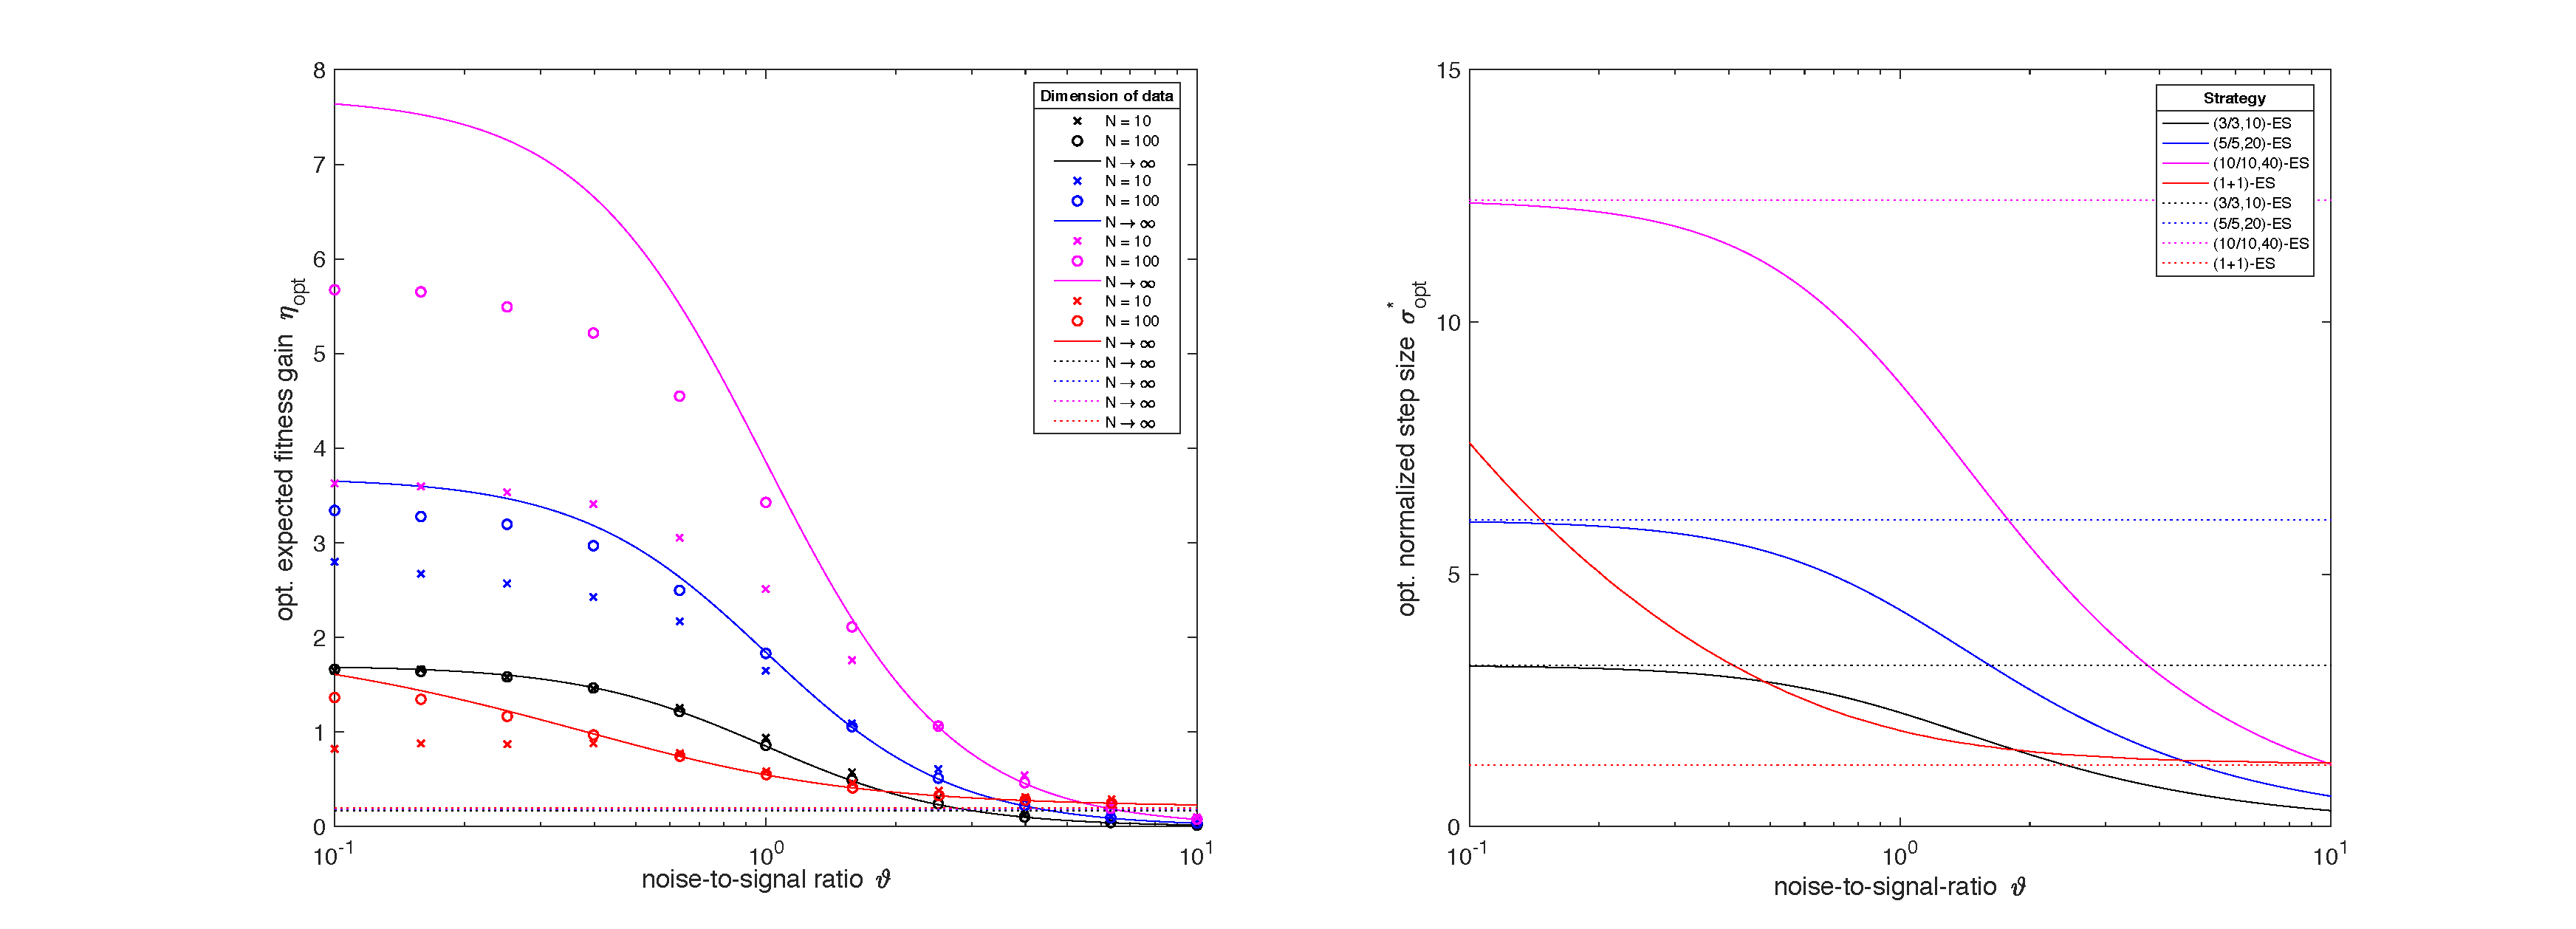
\includegraphics[width=1.0\linewidth]{opt_stepSize_fitGain_final.pdf}
    \caption{Expected values for surrogate model assisted $(\mu/\mu,\lambda)$-ES and (1+1)-ES plotted obtained by assuming independence of $\vartheta$ and $\sigma^*$}
\end{figure}
\end{itemize} 
\end{frame}

\begin{frame}{3.3 Observations}
\begin{itemize}
    \item Define \textbf{two speed-ups} for comparisons 
    \begin{itemize}
        \item $\text{speed-up}_{\text{self}}$: number of objective function calls used for a surrogate model assisted ES divided by that of the ES without surrogate model assistance (\textbf{$(\mu/\mu,\lambda)$-ES if not specified}). 
        \item $\text{speed-up}_{\text{model}}$: number of objective function calls used for surrogate model assisted (1+1)-ES divided by that of the surrogate model assisted $(\mu/\mu,\lambda)$-ES
    \end{itemize}     
    \item \textbf{Ideally}, $\text{speed-up}_{\text{self}} \overset{N\rightarrow\infty}{\rightarrow} \lambda$ as the surrogate model models the objective function exactly
    \item \textbf{In reality}, the  $\text{speed-up}_{\text{self}}$ degrades as $\varther$ increases. 
    
    When $N=10$, $\text{speed-up}_{\text{model}}$ is 2.4, 3.7, 4.7 for $(3/3,10)$-ES, $(5/5,20)$-ES, and $(10/10,40)$-ES respectively. 
    \item Overall the surrogate model assisted $(\mu/\mu,\lambda)$-ES achieves a larger opt. expected gain at a larger normalized step size relative to the surrogate model assisted (1+1)-ES. 
\end{itemize}
\end{frame}

%%%%%%%%%%%%%%%%%%%%%%%%%%%%%%%%%%%%%%%%%%%%%%%%%%%%%%%%%%%%%%%%%%%%%%%%%%%%%%%%%%
%%%%%%%%%%%%%%%%%%%%%%%%%%%%%%%%%%%%%%%%%%%%%%%%%%%%%%%%%%%%%%%%%%%%%%%%%%%%%%%%%%
% 4. Step size adaptation [Whole page]
\begin{frame}[plain,c]
%\frametitle{A first slide}
\begin{center}
\Huge 4. Step Size Adaptation
\end{center}
\end{frame}
\section{Step Size Adaptation}
%%%%%%%%%%%%%%%%%%%%%%%%%%%%%%%%%%%%%%%%%%%%%%%%
% 4.1 GP-mml-ES
\subsection{Cumulative step size adaptation}
\begin{frame}{4.1 Cumulative step size adaptation}
\begin{itemize}
    \item Even though the analysis in Analysis suggests a potential better performance for the surrogate-assisted $(\mu/\mu, \lambda)$-ES
    \item Problems with 
    \begin{itemize}
        \item No guarantee the step size of the strategy can be properly adapted
        \item The analysis is very inaccurate in finite dimensions
    \end{itemize}
    \item Use the GP surrogate model with dimension $N=10$, training size 40, length scale factor $8 \sigma \sqrt{N}$ and experiment with 
    \begin{itemize}
        \item \textbf{Linear sphere function}: $f(x) = (x^Tx)^{1/2}$ 
        \item \textbf{Quadratic sphere function}: $f(x) = x^Tx$ 
        \item \textbf{Cubic sphere function}: $f(x) = (x^Tx)^{3/2}$  
        \item \textbf{Schwefel Problem 1.2}: $f(x) = \sum_{i=1}^N(\sum_{j=1}^i x_j)^2$, a convex quadratic function with condition number of the Hessian $\approx175.1$
        \item \textbf{Quartic function}: $f(x) = \sum_{i=1}^{N-1} \left[ \beta(x_{i+1} -x_i^2)^2 + (1-x_i)^2 \right]$ where $\beta = 1$. For $\beta=100$ it becomes the Rosenbrock function with the condition number of the Hessian at the optimizer $>3,500$ (ill-conditioning problem).
    \end{itemize}
\end{itemize}
\end{frame}

%%%%%%%%%%%%%%%%%%%%%%%%%
\begin{frame}{4.1.1 Cumulative step size adaptation Alg.}

\begin{block}{Surrogate Model Assisted $(\mu/\mu,\lambda)$-ES (GP-$(\mu/\mu,\lambda)$-ES)}
 \footnotesize{
    \begin{algorithm}[H]
    \begin{algorithmic}[1]
        \STATE Initialize $c,d,E \left\lVert \mathcal{N}(0,I) \right\rVert,s^{(0)}$  using setting from Hansen [2]
        \WHILE{not terminate()} 
        	\FOR{$i=1,2,...,\lambda$}
        		\STATE Generate standard normally distributed $z_i^{(g)} \in \mathbb{R}^N $
        		\STATE Evaluate $x_{\text{centroid}}^{(g)} + \sigma^{(g)} z_i^{(g)}$ using the surrogate model, yielding $f_{\epsilon}(x_{\text{centroid}}^{(g)} + \sigma^{(g)} z_i)$
        	\ENDFOR
        	\STATE $z_{\text{step}}^{(g)} \leftarrow \frac{1}{\mu}\sum_{i=1}^{\mu} z_{i;\lambda}^{(g)}$
        	\STATE $x_{\text{centroid}}^{(g+1)} \leftarrow  x_{\text{centroid}}^{(g)} + \sigma^{(g)} z_{\text{step}}^{(g)}$ 
        	\STATE Evaluate $x_{\text{centroid}}^{(g+1)}$ using true objective function, yieding $f(x_{\text{centroid}}^{(g+1)})$
        	\STATE Update surrogate model by adding $(x_{\text{centroid}}^{(g+1)},f(x_{\text{centroid}}^{(g+1)}))$
        	\STATE $s^{(g)} \leftarrow (1-c)s + \sqrt{ c(2-c) \mu} z_{\text{step}}^{(g)}$
        	\STATE $\sigma^{(g+1)} \leftarrow \sigma^{(g)}  \text{exp} \left(\frac{c}{d} \frac{\left\lVert s^{(g)} \right\rVert} { E \left\lVert \mathcal{N}(0,I) \right\rVert} -1 \right )$
        	\STATE $g \leftarrow g + 1$
        \ENDWHILE
    \end{algorithmic}
    \end{algorithm}
}
\end{block}

\end{frame}

%%%%%%%%%%%%%%%%%%%%%%%%%
\begin{frame}{4.1.2 Experimental results}

\begin{figure}
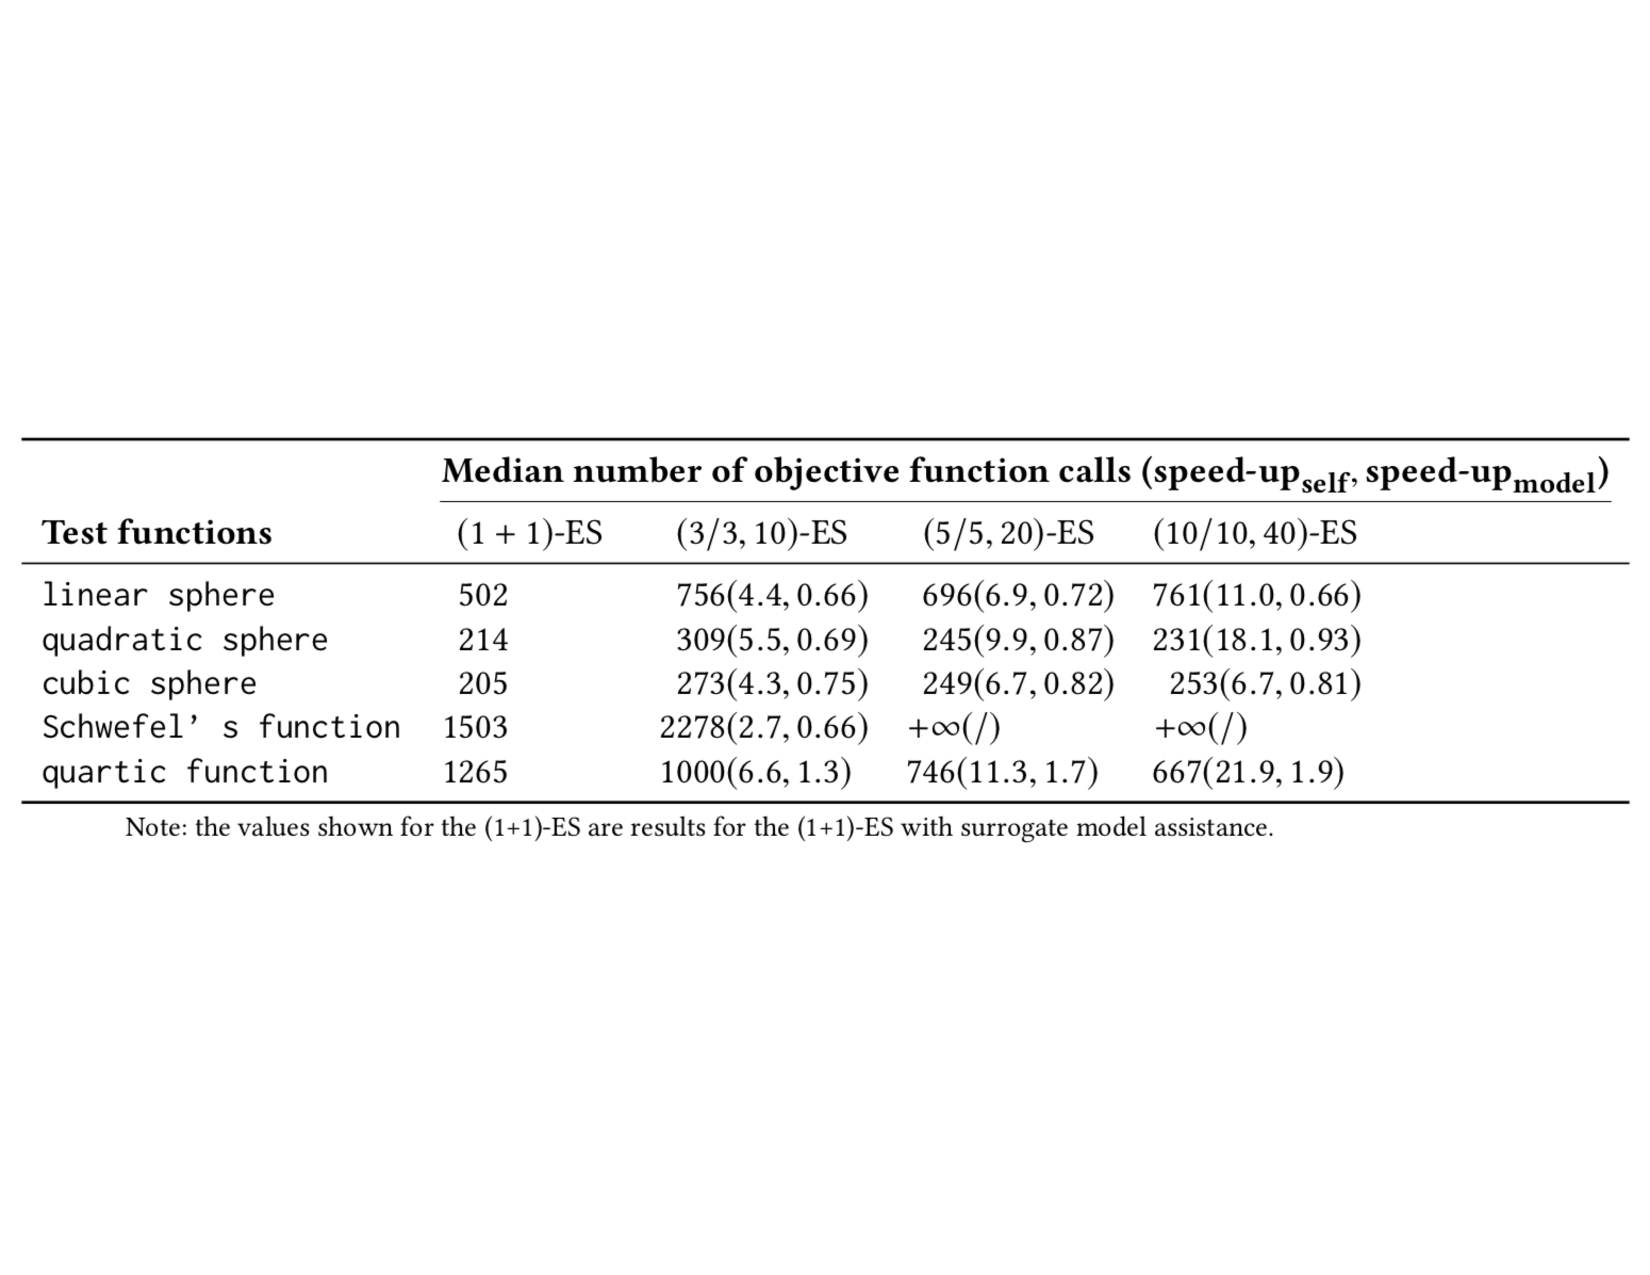
\includegraphics[width=1.0\linewidth]{tab-GP-mml-ES.pdf}
    \caption{Median test results and speed-ups of GP-$(\mu/\mu,\lambda)$-ES}
\end{figure}

\end{frame}
%%%%%%%%%%%%%%%%%%%%%%%%%
\begin{frame}{4.1.3 Interpretation}


\end{frame}


%%%%%%%%%%%%%%%%%%%%%%%%%%%%%%%%%%%%%%%%%%%%%%%%
% 4.2 GP-cross-ES
\subsection{Safeguard of plus-selection}

\begin{frame}{4.2 Safeguard of plus-selection}
\begin{itemize}
    \item The GP-$(\mu/\mu,\lambda)$-ES gives a success rate approximately equals to 0.5 for all population sizes used in all test functions
    \item How much to benefit if we can avoid or simply reject those bad steps
    \item A recent paper in surrogate model assisted ES considers (1+1)-ES where the step size is successfully adapted based on the success rate
    \begin{itemize}
        \item The step size is decreased if $f_\epsilon(y)>f(x)$ or $f(y)>f(x)$
    \end{itemize}
    \item Apply the same idea, propose a surrogate model assisted ES that is a cross between (1+1)-ES and $(\mu/\mu,\lambda)$-ES ( referred to as GP-cross-ES)
        \begin{itemize}
            \item Safeguard of plus-selection -- discards bad steps, i.e., rejects offspring inferior to its parent
            \item Decrease step size if $f_\epsilon(y)>f(x_{\text{centroid}})$
        \end{itemize}
        
\end{itemize}
\end{frame}

%%%%%%%%%%%%%%%%%%%%%%%%%
\begin{frame}{4.2.1 Safeguard of plus-selection Alg.}
\begin{block}{Surrogate model assisted ES with plus-selection (GP-cross-ES)}
 \footnotesize{
    \begin{algorithm}[H]
    \begin{algorithmic}[1]
        \STATE Initialize $c,d,E \left\lVert \mathcal{N}(0,I) \right\rVert,s^{(0)}$  using setting from Hansen [2], $D \leftarrow 0.72$
       \WHILE{not terminate()} 
    	\FOR{$i=1,2,...,\lambda$}
    		\STATE Generate standard normally distributed $z_i^{(g)} \in \mathbb{R}^N $
    		% \STATE $y_i^{(g)} \leftarrow x_{\text{centroid}}^{(g)} + \sigma^{(g)} z_i$
    		\STATE Evaluate $x_{\text{centroid}}+ \sigma^{(g)} z_i^{(g)}$ using the surrogate model, yielding $f_{\epsilon}(x_{\text{centroid}} + \sigma^{(g)} z_i^{(g)})$
    	\ENDFOR
    	\STATE $z_{\text{step}}^{(g)} \leftarrow \frac{1}{\mu}\sum_{i=1}^{\mu} z_{i;\lambda}^{(g)}$
    	\STATE $y  \leftarrow  x_{\text{centroid}} + \sigma^{(g)} z_{\text{step}}^{(g)}$ 
    	\STATE Evaluate $y$ using true objective function, yielding $f(y)$
    	\STATE Update surrogate model by adding $(y,f(y))$
    	\IF{$f(x_{\text{centroid}}) < f(y)$ (occurrence of a bad step)}
    		\STATE $\sigma \leftarrow \sigma D$
    	\ELSE
    		\STATE $ x_{\text{centroid}} \leftarrow y $. Update $s^{(g)},\sigma^{(g+1)}$ using CSA \hfill$\blacktriangleright$\Comment{plus-selection} % comment
    	\ENDIF
    	\STATE $g \leftarrow g + 1$
    \ENDWHILE
    \end{algorithmic}
    \end{algorithm}
}
\end{block}
\end{frame}

%%%%%%%%%%%%%%%%%%%%%%%%%
\begin{frame}{4.2.2 Experimental results}

\begin{figure}
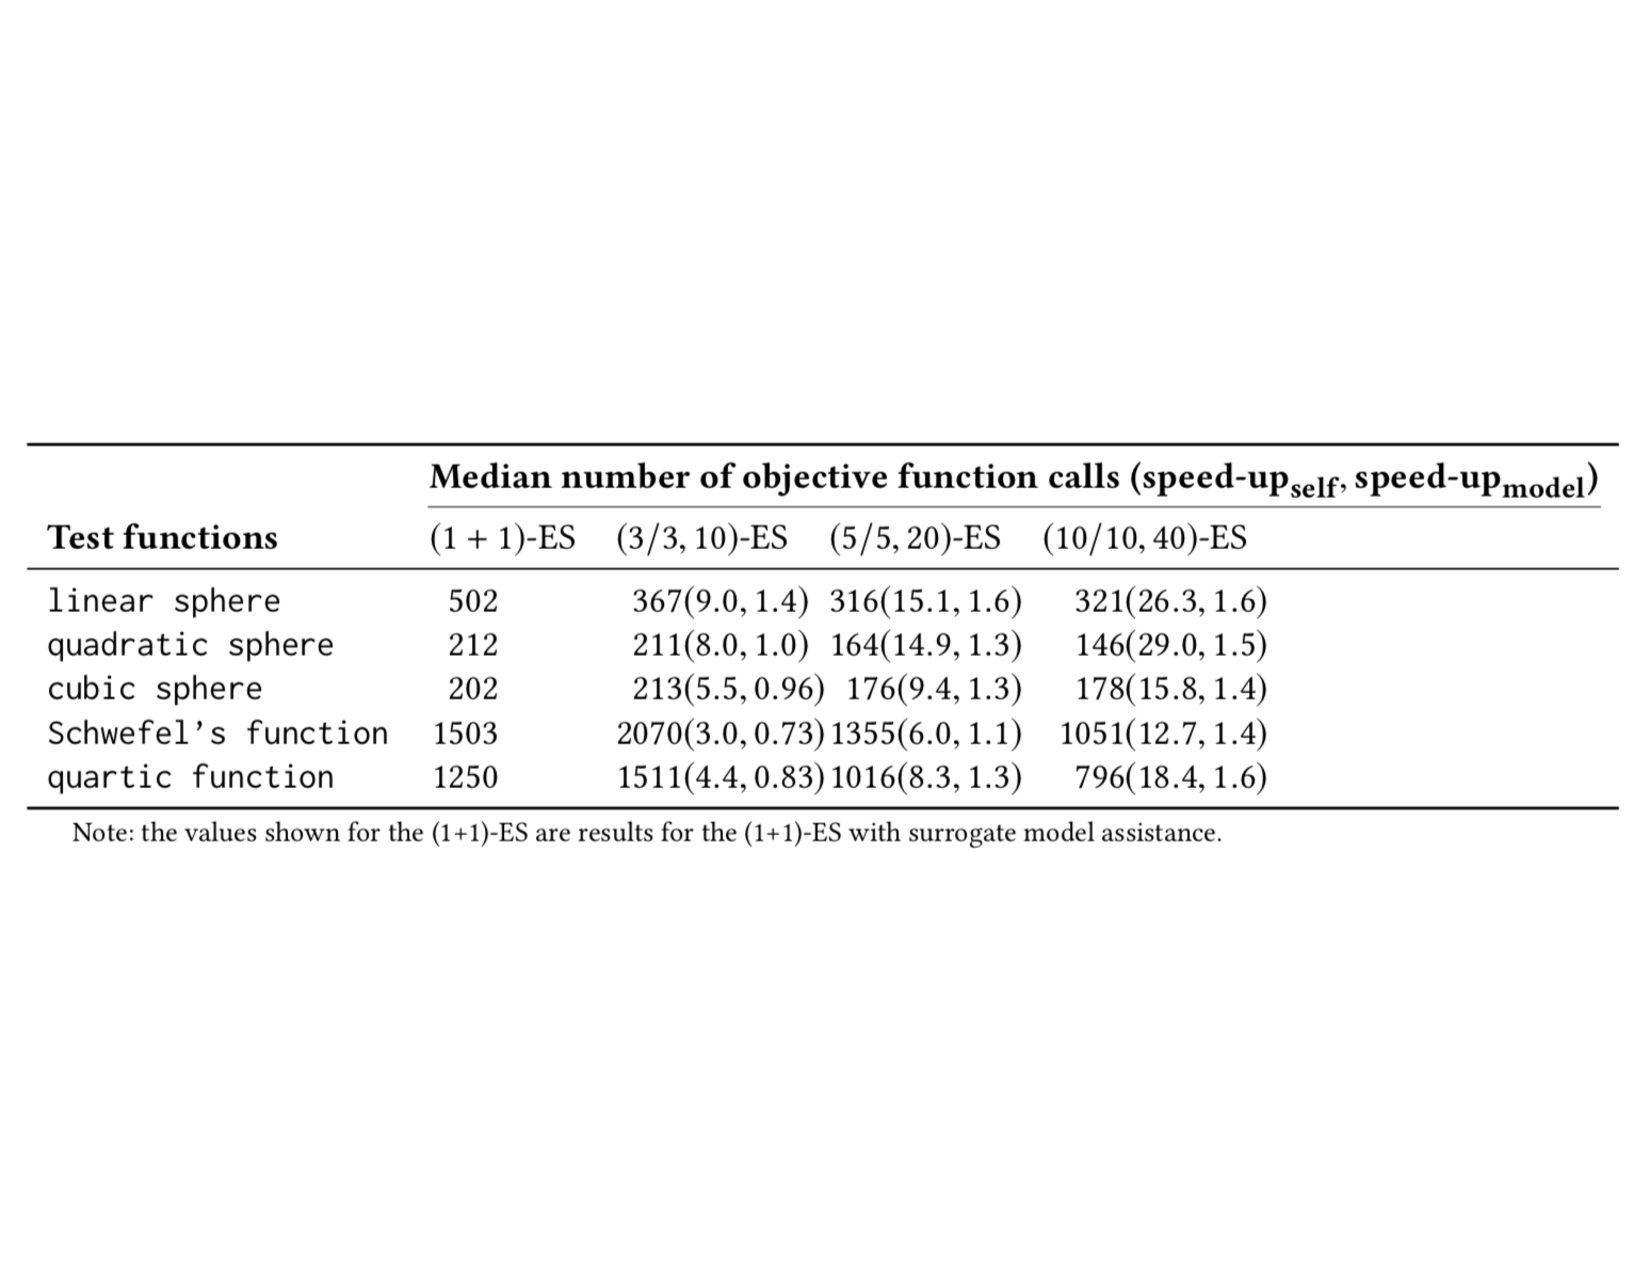
\includegraphics[width=1.0\linewidth]{tab-GP-cross-ES.pdf}
    \caption{Median test results and speed-ups of GP-cross-ES}
\end{figure}


\end{frame}

%%%%%%%%%%%%%%%%%%%%%%%%%
\begin{frame}{4.2.3 Interpretation}


\end{frame}

%%%%%%%%%%%%%%%%%%%%%%%%%%%%%%%%%%%%%%%%%%%%%%%%%%%%%%%%%%%%%%%%%%%%%%%%%%%%%%%%%%
%%%%%%%%%%%%%%%%%%%%%%%%%%%%%%%%%%%%%%%%%%%%%%%%%%%%%%%%%%%%%%%%%%%%%%%%%%%%%%%%%%
% 5. Conclusion [Whole page]
\begin{frame}[plain,c]
%\frametitle{A first slide}
\begin{center}
\Huge 5. Conclusion and Future Work
\end{center}
\end{frame}
\section{Conclusion and Future Work}
%%%%%%%%%%%%%%%%%%%%%%%%%%%%%%%%%%%%%%%%%%%%%%%%
% 5.1 Conclusion
\begin{frame}{5.1 Conclusion}
  \begin{itemize}
  \item
    We analyzed the proposed GP-$(\mu/\mu,\lambda)$-ES using the simple model for surrogate modelling approach
    \begin{itemize}
        \item Excepted $\text{speed-up}_{\text{self}}\rightarrow \lambda$ if the surrogate model is accurate
    \end{itemize}
  \item
    We experimented the GP-$(\mu/\mu,\lambda)$-ES on five test functions and compare the results with the surrogate model assisted (1+1)-ES
    \begin{itemize}
        \item Experimental $\text{speed-up}_{\text{self}}$ is a factor of 4 smaller than expected. 
    \end{itemize}
  \item
    Tried to interpret the results and proposed GP-cross-ES taking benefit of plus-selection.
    \begin{itemize}
        \item Step size is successfully adapted in all runs
        \item Overall $\text{speed-up}_{\text{model}}$ about 1.4 to 1.6 for a population size $\lambda \geq 20$ in all five test functions
    \end{itemize}
  \end{itemize}
  
\end{frame}

\begin{frame}{5.2 Future Work}
  \begin{itemize}
  \item
    Study the behaviours of the surrogate assisted CMA-ES using the same simple model that potentially help handle ill-conditioned problems
  \item
    Future goals include
    \begin{itemize}
        \item Understanding the effect of length scale parameter in the Gaussian Process model 
        \item Potential length scale adaptation mechanism
        \item Surrogate accuracy control
    \end{itemize}

  \end{itemize}
  
\end{frame}
%%%%%%%%%%%%%%%%%%%%%%%%%%%%%%%%%%%%%%%%%%%%%%%%%%%%%%%%%%%%%%%%%%%%%%%%%%%%%%%%%%%%%%%%%%
% 6. References
\begin{frame}{References}
%   \begin{itemize}
%   \item
%     Study the behaviours of the surrogate assisted CMA-ES using the same simple model that potentially help handle ill-conditioned problems
%   \item
%     Future goals includes 
%     \begin{itemize}
%         \item Understanding the effect of length scale parameter in the Gaussian Process model 
%         \item Potential length scale adaptation mechanism
%         \item Surrogate accuracy control
%     \end{itemize}

%   \end{itemize}
  
\end{frame}

% All of the following is optional and typically not needed. 
\appendix
\section<presentation>*{\appendixname}
\subsection<presentation>*{References}

\begin{frame}[allowframebreaks]
  \frametitle<presentation>{For Further Reading}
    
  \begin{thebibliography}{10}
    
  \beamertemplatebookbibitems
  % Start with overview books.

  \bibitem{Author1990}
    A.~Author.
    \newblock {\em Handbook of Everything}.
    \newblock Some Press, 1990.
 
    
  \beamertemplatearticlebibitems
  % Followed by interesting articles. Keep the list short. 

  \bibitem{Someone2000}
    S.~Someone.
    \newblock On this and that.
    \newblock {\em Journal of This and That}, 2(1):50--100,
    2000.
  \end{thebibliography}
\end{frame}



%------------------------------------------------

\begin{frame}
\Huge{\centerline{The End}}
\end{frame}

%----------------------------------------------------------------------------------------\end{document}

\end{document}